\documentclass[conference]{IEEEtran}
% If the IEEEtran.cls has not been installed into the LaTeX system files,
% manually specify the path to it.  e.g.
% \documentclass[conference]{./IEEEtran}

% Add and required packages here
\usepackage{graphicx,times,amsmath, fontenc, epstopdf}
\usepackage[utf8]{inputenc}
\usepackage[T1]{fontenc}

% Correct bad hyphenation here
\hyphenation{op-tical net-works semi-conduc-tor IEEEtran}

% To create the author's affliation portion using \thanks
\IEEEoverridecommandlockouts

\textwidth 178mm
\textheight 239mm
\oddsidemargin -7mm
\evensidemargin -7mm
\topmargin -6mm
\columnsep 5mm

\begin{document}

% Paper title: keep the \ \\ \LARGE\bf in it to leave enough margin.
\title{\ \\ \LARGE\bf Combining Clustering and FSM models \\ for Adaptive Level Generation\thanks{Jorge Diz and David Camacho are with the Computer Science Department, Escuela Politécnica Superior, Universidad Autónoma de Madrid. c/ Francisco Tomás y Valiente 11, 28049 Madrid, Spain. (email: {\tt jorge.diz@estudiante.uam.es} and {\tt david.camacho@uam.es})}}

\author{Jorge Diz Pico, David Camacho}

% Uncomment out the following line for invited papers
%\specialpapernotice{(Invited Paper)}

% Make the title area
\maketitle

\begin{abstract}
Content generation has been widely used in gaming
to offer virtually infinite replayability.
Its combination with adaptive techniques also provides a tighter fit between
results and gameplay.
A new approach for procedural level generation
is presented based on a combination of clustering and finite state machines.
The method has been designed and deployed as an entry for the 
Level Generation track of the Mario AI Championship.
The implemented architecture is shown to provide
great flexibility for both refinement and
extension to other games, and the
experimental results are shown to prove
the validity of this approach. 

\end{abstract}

% No keywords

\section{Introduction}
Procedural level generation, in one way or another, has been present since the inception of games history. Initially, its role was to make up for lack of storage memory for levels by creating them on the fly. It soon revealed its potential to make a game ``infinite'' by presenting the player with a fresh envinroment every time, a quality best exemplified in early 1980s adventure classic \textit{Rogue} (Toy and Wichman). Since then, it has been featured prominently in many commercially successful games such as the roleplaying series \textit{Diablo} (developed by Blizzard, 1996) or the exploration-based \textit{Minecraft} (Mojang, 2009). It's uses have even expanded to terrain creation \cite{rodenparberry2004} or quest design \cite{mmorpg06}.
Mario AI Championship
Lately, some of these techniques have been coupled with adaptive algorithms to make the content generated not only random but also tied to the characteristics of the player. One of the most remarkable examples is the \textit{``AI Director`''} found in \textit{Left 4 Dead 2} (Valve, 2009), that even goes as far as to adapt the challenges while the level is played if it finds the player low on health or ammunition \cite{l4d09}.

In this work, a novel approach to adaptive level generation is presented after testing it on the platform provided by the Mario AI Championship. Previous instances of this competition have featured many worthy techniques \cite{mario2010}; inspired by them, an architecture was devised that can prove not only equally valid but quite flexible for expansion and adaptation as well.

\section{Methodology}

The presented approach tries to offer a new insight into adaptively generating random levels. It is comprised of two main parts: a data-driven clustering process (mostly offline), and a finite state machine execution (online). A third layer, a library of functions that actually build the level, serves as the link between the adaptive generator system and the game API. 

\begin{figure*}[htp]
\centerline{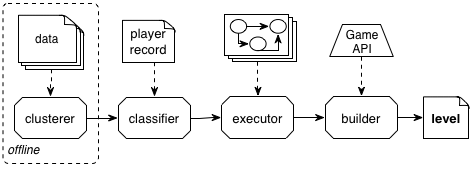
\includegraphics[width=1.2\columnwidth]{layers.png}}
\caption{Layers and modules of the proposed architecture}
\label{layers}
\end{figure*}

\subsection{Clustering}

The topmost layer undertakes a clustering process on data collected from user play. This approach bases the decisions on empirical metrics and avoids overguessing. This execution can be run offline once and then stored for use afterwards, reducing the computational load on the level generation process. It only needs to be rerun when new samples are collected, to refine and recheck the clustering.

The suggested method for collecting samples is to present a vast array of different players with roughly similar levels (ideally, the same). Having them face comparable challenges makes possible to extrapolate on their gameplay style. So as to not overtrain on a particular player, it is recommended to keep just one significant sample per player. Those collections are then clustered as mentioned before.

Now, when a new player comes to the game, he is made to play a test level in the same vein as the ones used in the aforementioned process. The records of his gameplay are fed to a clusterer that will assign him to one of groups found.

It must be noted that the classification shown here is the most basic approach. Clustering could be further refined, perhaps selecting different parameters at different executions, obtaining the player's position along two different axis; or supporting it with additional inputs like the preferred difficulty. There have been successful experiences working with rhythmic patterns \cite{rhythm09} and identifying emotional response from frustation or challenge \cite{shaker10}.

\subsection{Finite state machines}

Once the player has been identified as belonging to a given group, this association is used to further assign him an automaton. This is done on a one-to-one basis: each group has a finite state machine modeled and tailored to its detected needs, defined upon inspection of their characteristic metrics.

These machines have each their own states and transitions, but most importantly, those transitions are defined as probabilistic. Traversing an automaton is done by picking between the next available states from the current one, weighted by the probability associated to that movement. This feature adds the random component needed to keep the levels generated fresh and unique every time, even though the automata themselves are always the same.

This probabilistic nature in which the next state is only based on the current one makes the automata a model of a Markov chain of order one. Statistical considerations can be calculated on the overall probability that each state is reached when the automaton is traversed, opening the door to reducing frequencies in a controlled manner.

To further enforce modularity, the automata sit on top of a builder layer that acts as an API through its several level constructing functions. Each state delegates its world-building function to this layer, preventing code repetition on the states and promoting code sharing and reuse.

A diagram of the flow is shown in figure~\ref{layers}.

\section{Results}

Work was started by collecting data from many different players. Each participant was asked to play one of the levels generated by the standard, random algorithm found in the Mario AI Championship platform, and return the resulting records. Social networks and word of mouth were used to recruit volunteers, managing to get 115 different user profiles at the time of this article.


\begin{table}
\begin{center}
\renewcommand{\arraystretch}{1.3}
\caption{Log Likelihood of the different clusterers}
\label{tableloglikelihood}
\begin{tabular}{|c|c|}
\hline
HierarchicalCluster: & 79.28\\
\hline
FarthestFirst: & 80.70\\
\hline
XMeans: & 84.83 \\
\hline
SimpleKMeans: & 84.03 \\
\hline
EM: & 86.64 \\
\hline
\end{tabular}
\end{center}
\end{table}

Several clustering algorithms were then tried to detect the different playstyles: \textit{HierarchicalClusterer}, \textit{FarthestFirst}, \textit{XMeans}, \textit{SimpleKMeans} and \textit{EM}.
All algorithms, except EM, were wrapped in MakeDensityBasedClusters to compare their log likelihoods, which can be checked above in table~\ref{tableloglikelihood} .The best value was obtained with \textit{Expectation-Maximization}, with \textit{SimpleKMeans} and \textit{XMeans} close behind. 

The parameters wre configured as standard for the Weka library, except for the number of clusters, that was set to three after several tries. There were two factors to balance: a bigger number meant a better personalization; a small number meant sometimes obtaining clusters with only a handful of players. Four and five clusters were consistently distorting the personality of the clusters (no meaningful conclusions could be extracted from them) and therefore were discarded.


\begin{table*}
\begin{center}
\renewcommand{\arraystretch}{1.7}
\caption{Clusters and their parameters ranks}
\label{tableparameters}
\begin{tabular}{|c|c|c|}
\hline
	Nickname & highest & lowest
\\
\hline
	``explorers'' 
	& \begin{minipage}[c]{0.7\columnwidth}GoombasKilled, aimlessJumps, coinBlocksDestroyed, coinsCollected, completionTime, duckNumber, emptyBlocksDestroyed, enemyKillByFire, jumpsNumber, percentageBlocksDestroyed, percentageCoinBlocksDestroyed, percentageEmptyBlocksDestroyed, percentagePowerBlockDestroyed, timeRunningLeft, timeRunningRight, timeSpentDucking, timesPressedRun, timesSwitchingPower, totalEmptyBlocks, totalTime, totalTimeFireMode, totalTimeLargeMode, totalTimeLittleMode, totalPowerBlocks\end{minipage}
	& \begin{minipage}[c]{0.7\columnwidth}timeSpentRunning\end{minipage}
\\
\hline
	``speeders''
	& \begin{minipage}[c]{0.7\columnwidth}timeSpentRunning, timesofDeathByGoomba\end{minipage}
	& \begin{minipage}[c]{0.7\columnwidth}GoombasKilled, aimlessJumps, coinBlocksDestroyed, coinsCollected, completionTime, duckNumber, emptyBlocksDestroyed, enemyKillByFire, jumpsNumber, percentageBlocksDestroyed, percentageCoinBlocksDestroyed, percentageEmptyBlocksDestroyed, percentagePowerBlockDestroyed, timeRunningLeft, timeRunningRight, timeSpentDucking, timesPressedRun, timesSwitchingPower, totalCoinBlocks, totalCoins, totalEmptyBlocks, totalEnemies, totalTime, totalTimeFireMode, totalTimeLargeMode, totalPowerBlocks\end{minipage}
\\
\hline
	``intermediates''
	& \begin{minipage}[c]{0.7\columnwidth}totalCoinBlocks, totalCoins, totalEnemies\end{minipage}
	& \begin{minipage}[c]{0.7\columnwidth}timesofDeathByGoomba, totalTimeLittleMode\end{minipage}
\\
\hline
\end{tabular}
\end{center}
\end{table*}

The Mario AI Championship platform stores 45 metrics of user gameplay, mostly related to time spent performing actions and items collected. But some of them were filtered due to the characteristics of the sample level that the platform generates. There are no flower piranhas, no gaps, and no enemies other than goombas. Therefore, all the following metrics were excluded from the study and custering, since their value was always zero: \textit{ArmoredTurtlesKilled}, \textit{CannonBallKilled}, \textit{ChompFlowersKilled}, \textit{GreenTurtlesKilled}, \textit{RedTurtlesKilled}, \textit{enemyKillByKickedShell}, \textit{kickedShells}, \textit{timesofDeathByArmoredTurtle}, \textit{timesofDeathByCannonBall}, \textit{timesofDeathByChompFlower}, \textit{timesofDeathByFallingIntoGap}, \textit{timesofDeathByGreenTurtle}, \textit{timesofDeathByJumpFlower}, \textit{timesofDeathByRedTurtle}.

As mentioned, with three clusters a ``personality'' for their players could be inferred from their values. One of the them was identifiable by the high number of blocks broken and enemies killed, as well as long completion times. The users in this group were nicknamed ``explorers''. Another cluster was characteristic for its quick completion time, long use of running mode, and disregard for powerups. They were nicknamed ```speeders''. Finally, the remaining cluster, presenting a more neutral set of attributes, were nicknamed ``intermediates''. A full classification of the parameters can be consulted in table~\ref{tableparameters}. Figure~\ref{wekaplot} shows a plot of one of the parameters, \textit{timeRunningLeft} (some jittering was added for easier visualization). This value can be interpreted as a measure of backtracking to interact with missed elements, and is shown here to be quite crucial in telling apart the clusters. 

\begin{figure}[htp]
\centerline{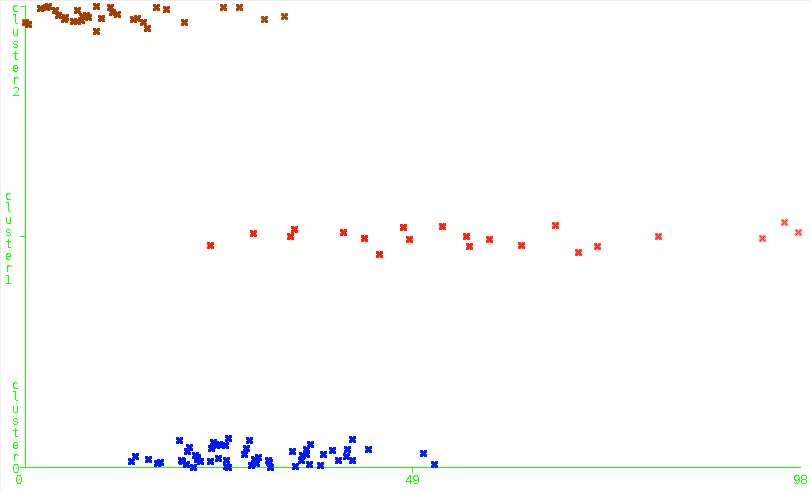
\includegraphics[width=0.9\columnwidth]{timeRunningLeft_.png}}
\caption{timeRunningLeft plotted against cluster membership}
\label{wekaplot}
\end{figure}

Per this observation, and reflecting on the meaning of those user profiles, three automata were designed, attending to the inferred needs of those clusters. For example, speeders may frown upon blocks of ``stairs'' because they often force a stop of the running flow. Similarly, explorers tend to enjoy double rows of blocks, an aspect overlooked by the other types of players. 

\begin{figure}[htp]
\centerline{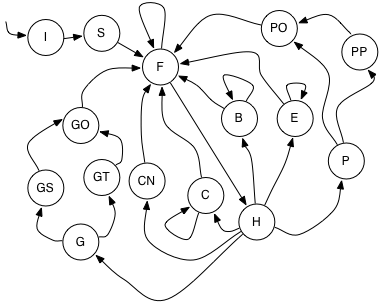
\includegraphics[width=0.75\columnwidth]{automaton.png}}
\caption{Simplified automaton designed for intermediates (probabilities removed for clarity)}
\label{automaton}
\end{figure}

\begin{figure}[htp]
\centerline{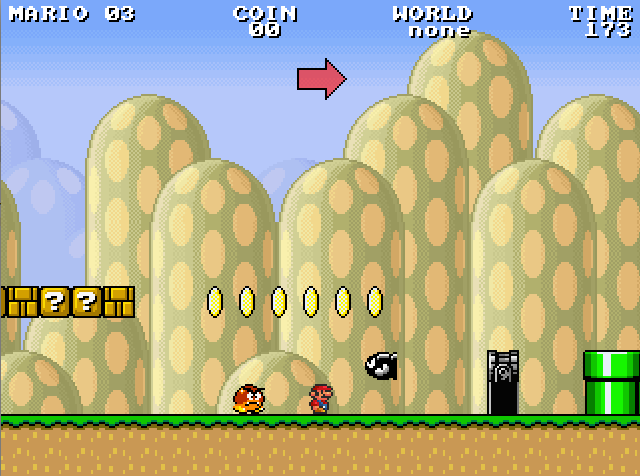
\includegraphics[width=0.75\columnwidth]{screenshot.png}}
\caption{Screenshot of a random level generated by the above automaton}
\label{screenshot}
\end{figure}

Figure~\ref{automaton} and figure~\ref{screenshot} show a suggested simple automaton for intermediates, with all basic elements present, and a level generated by it, respectively. Transition probabilities are not shown for size constraints and clarity. Dashed states are ``empty'', that is, they place no elements on the level and exist only for convenience in design.

The general flow of this automaton is to build its initial platform ({\bf S}), some flat land ({\bf F}) and then cyclically go from the global hub ({\bf H}) into branches, each representing a different part of the scene that could be built. At the end of each branch, some flat land is added for buffering. Lots of different elements immediately adjacent resulted in not only visually unpleasant, bur rhythmically dissonant segments and severely hurt pacing. Spacing between them helped to offer a smoother cadence.

Let's focus now, for example, on the branch for \textit{gaps}. State {\bf G} serves as entry point for all kinds of gaps, accesible from the hub {\bf H}. This transition provides an opportunity to regulate the overall frequency of gaps in our level. Then, two states bifurcate the way: {\bf GS} places a gap with stairs surrounding it, while {\bf GT} places a regular, bare gap. It's here when the individual probability of each gap can be weighted. Finally, both of them go out through dummy state {\bf GO} (for {\it gap out}).

In this case {\bf GO} only goes to {\bf F} as mentioned before, but it could be made to loop on itself. This is how blocks ({\bf B}), coins ({\bf C}) or enemies ({\bf E}) are implemented. Each pass through the state places but one sprite on the level. It's the loop that creates a row. Tuning the probability moderates the average number of coins (for instance) that are expected to be found on a given strike.

\section{Conclusions}

Records belonging to the three different clusters were fed to the algorithm, and playtest showed that each of the levels generated had the capacity of feeling different to the others.

The architecture shown in this paper offers great expansion potential. Its modularity expressed through several layers diminishes the interferences of the different parts. For instance, new player types may be detected in the clustering layer, and the changes in the automata layer would be minimal -- just adding a new FSM that does not break existing functionality. Similarly, changes in an existing FSM would not affect neither the clustering layer nor the other FSMs of the system. Furthermore, new states and transitions may be added without the need for modifications on the underlying library of builder functions they call upon.

In summary, as different preferences and goals are accounted for, the approach allows for great flexibility on the process followed for each user. Reducing the space of all possible players into a small number of aggregated playstyles also tones down the number of needed automata as to be few enough to be designed by hand. Manually crafting the states and transitions improves the overall arching flow, per the control over sequentially adjacent ``chunks'' of the level. Albeit keeping its characteristic randomness, the levels are ensured to have an orderly sense instead of being just a messy sequence of pieces.

\subsection*{Future work}

One of the most promising aspects of the presented architecture is its flexibility to be enhanced in several ways. We consider combination with evolutionary techniques to be the most rewarding path. Even though determining the existence of transitions (links) between states can be left to the designer's choice, the actual weight of those transitions can be easily obtained by evolution, pondering user feedback from the level play until finding a fine-tuned balance. Similarly, players can be better represented by percentages of similarity to given clusters than by hard assignment. Using those percentages, the automata can be mixed and matched to offer a more personalized experience, by encoding them as grammars and using grammatical evolution.

\section*{Acknowledgments}
This work has been supported by the
Spanish Ministry of Science and Innovation under grant
TIN2010-19872 (ABANT).

% Trigger a \newpage just before a given reference number in order to
% balance the columns on the last page.  Adjust the value as needed;
% it may need to be readjusted if the document is modified later.
%\IEEEtriggeratref{8}
% The "triggered" command can be changed if desired:
%\IEEEtriggercmd{\enlargethispage{-5in}}

% The references section can either be generated by hand or by an
% automatic tool like BibTeX.  If using BibTex, use the standard IEEEtran
% bibliography style.
\bibliographystyle{IEEEtran.bst}
%
% The argument to \bibliography is/are the name(s) of your BibTeX file(s)
% that contains string definitions and bibliography database(s).
\bibliography{IEEEabrv,jorgedizpico}
%
% If you generate the bibliography by hand, or if you copy in the
% resultant .bbl file, set the second argument of \begin to the number of
% references in the bibliography (used to reserve space for the reference
% number labels box).

%\begin{thebibliography}{3}
%\bibitem{book}
%A.~Great, \emph{This is the book title}.\hskip 1em plus 0.5em minus 0.4em\relax
%  This is the name of the publisher, 2006.

%\bibitem{conf}
%F.~Author, S.~Author, and T.~NonRelatedAuthor, ``This is the paper title,'' in
%  \emph{This is the proceedings title}, 2008, pp. 1--8.

%\bibitem{article}
%B.~Myself, ``This is the title of the journal article,'' \emph{This is the name
%  of the journal}, pp. 1--30, 2007.
%\end{thebibliography}

% That's all folks...
\end{document}
